%%%%%%%%%%%%%%%%%%%%%%%%%%%%%%%%%%%%%%%%%
% Journal Article
% LaTeX Template
% Version 1.4 (15/5/16)
%
% This template has been downloaded from:
% http://www.LaTeXTemplates.com
%
% Original author:
% Frits Wenneker (http://www.howtotex.com) with extensive modifications by
% Vel (vel@LaTeXTemplates.com)
%
% License:
% CC BY-NC-SA 3.0 (http://creativecommons.org/licenses/by-nc-sa/3.0/)
%
%%%%%%%%%%%%%%%%%%%%%%%%%%%%%%%%%%%%%%%%%

%----------------------------------------------------------------------------------------
%	PACKAGES AND OTHER DOCUMENT CONFIGURATIONS
%----------------------------------------------------------------------------------------

\documentclass[twoside,twocolumn]{article}

\usepackage{blindtext} % Package to generate dummy text throughout this template

\usepackage[sc]{mathpazo} % Use the Palatino font
\usepackage[T1]{fontenc} % Use 8-bit encoding that has 256 glyphs
\linespread{1.05} % Line spacing - Palatino needs more space between lines
\usepackage{microtype} % Slightly tweak font spacing for aesthetics

\usepackage[english]{babel} % Language hyphenation and typographical rules

\usepackage[hmarginratio=1:1,top=32mm,columnsep=20pt]{geometry} % Document margins
\usepackage[hang, small,labelfont=bf,up,textfont=it,up]{caption} % Custom captions under/above floats in tables or figures
\usepackage{booktabs} % Horizontal rules in tables

\usepackage{lettrine} % The lettrine is the first enlarged letter at the beginning of the text

\usepackage{enumitem} % Customized lists
\setlist[itemize]{noitemsep} % Make itemize lists more compact

\usepackage{abstract} % Allows abstract customization
\renewcommand{\abstractnamefont}{\normalfont\bfseries} % Set the "Abstract" text to bold
\renewcommand{\abstracttextfont}{\normalfont\small\itshape} % Set the abstract itself to small italic text

\usepackage{titlesec} % Allows customization of titles
\renewcommand\thesection{\Roman{section}} % Roman numerals for the sections
\renewcommand\thesubsection{\roman{subsection}} % roman numerals for subsections
\titleformat{\section}[block]{\large\scshape\centering}{\thesection.}{1em}{} % Change the look of the section titles
\titleformat{\subsection}[block]{\large}{\thesubsection.}{1em}{} % Change the look of the section titles

\usepackage{fancyhdr} % Headers and footers
\pagestyle{fancy} % All pages have headers and footers
\fancyhead{} % Blank out the default header
\fancyfoot{} % Blank out the default footer
\fancyhead[C]{} % Custom header text
\fancyfoot[RO,LE]{\thepage} % Custom footer text

\usepackage{titling} % Customizing the title section

\usepackage{hyperref} % For hyperlinks in the PDF

\usepackage{amsmath}
\newcommand*\diff{\mathop{}\!\mathrm{d}}
\newcommand*\Diff[1]{\mathop{}\!\mathrm{d^#1}}

\usepackage{graphicx}
\graphicspath{ {./images/} }

%----------------------------------------------------------------------------------------
%	TITLE SECTION
%----------------------------------------------------------------------------------------

\setlength{\droptitle}{-4\baselineskip} % Move the title up

\pretitle{\begin{center}\Huge\bfseries} % Article title formatting
\posttitle{\end{center}} % Article title closing formatting
\title{Swap Pallet} % Article title
\author{%
\textsc{Parami Devs} % Your name
\normalsize \href{mailto:devs@parami.io}{devs@parami.io} % Your email address
%\and % Uncomment if 2 authors are required, duplicate these 4 lines if more
%\textsc{Jane Smith}\thanks{Corresponding author} \\[1ex] % Second author's name
%\normalsize University of Utah \\ % Second author's institution
%\normalsize \href{mailto:jane@smith.com}{jane@smith.com} % Second author's email address
}
\date{\today} % Leave empty to omit a date
\renewcommand{\maketitlehookd}{%
\begin{abstract}
\noindent We implement swap pallet for assets pricing and trading
using the constant product market maker model (aka, $x\times\,y=k$ model)\cite{ref1},
and additional farming algorithm to encourage investors to add liquidity into the pool.
\end{abstract}
}

%----------------------------------------------------------------------------------------

\begin{document}

% Print the title
\maketitle

%----------------------------------------------------------------------------------------
%	ARTICLE CONTENTS
%----------------------------------------------------------------------------------------

\section{Introduction}

\lettrine[nindent=0em,lines=3]{O}ur swap algorithm is following the design of Uniswap v1\cite{ref2},
the swap pallet provides an interface for seamless exchange of assets on Parami blockchain.
By eliminating unnecessary forms of rent extraction and middlemen it allows faster,
more efficient exchange.
Where it makes tradeoffs, decentralization, censorship resistance,
and security are prioritized.

In additional, the swap pallet provide the ability to farm assets with a farming curve.
To do so, inspired by Uniswap v3, the swap pallet use NFT for liquidity provider tokens.

%------------------------------------------------

\section{Goals}

With the design of Parami Protocol, the goals of the swap pallet are:
\begin{itemize}
    \item Provide pricing for each KOL NFT fragment / DAO coin
    \item Join liquidity polls to collect fess on pairs
    \item Liquidity-sensitive automated pricing
    \item Liquidity-based farming of assets
    \item Low fee cost
\end{itemize}

% Text requiring further explanation\footnote{Example footnote}.

%------------------------------------------------

\begin{figure}[h]
    \centering
    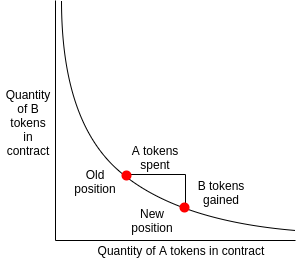
\includegraphics[width=0.3\textwidth]{xyk}
\end{figure}

\section{Implementation}

\subsection{Pricing}

To achieve the goals, the swap pallet
implementated constant product formula\cite{ref3}
for Liquidity-sensitive automated pricing.

Following the $x\times\,y=k$ model,
when sell $\Delta\,x$ tokens,
the user will get $\Delta\,y$ tokens,
such that $x\times\,y=(x+\Delta\,x)\times(y-\Delta\,y)$,
thus the price ($\Delta\,x/\Delta\,y$) is the function of $x/y$.

With a fee $\rho=0.003$, the token reserves are updated as follows:
\begin{align*}
    {x}'_{\rho} & =x+\Delta\,x=(1+\alpha)x=\frac{1+\beta(\frac{1}{\gamma}-1))}{1-\beta}x, \\
    {y}'_{\rho} & =y-\Delta\,y=\frac{1}{1+\alpha\gamma}y=(1-\beta)y
\end{align*}
where $\alpha=\frac{\Delta\,x}{x}$, $\beta=\frac{\Delta\,y}{y}$, $\gamma=1-\rho$.

When get input price, with 0.3\% fee,
the price is implemented as follows:
\[
    (997*\Delta\,x*y)/(1000*x+997*\Delta\,x)
\]

When get output price, with the same fee,
the price is implemented as follows:
\[
    (1000*x*\Delta\,y)/(997*(y-\Delta\,y))+1
\]

\subsection{Liquidity}

An investor can mint liquidity by depositing both AD3 and asset.

When add liquidity,
it takes as input $\Delta\,e>0$ and updates the state as follows:
\[
    (e,t,l)\mathop{\to}^{\Delta\,e}({e}',{t}',{l}')
\]
where
\begin{align*}
    {e}''  & = e+\Delta\,e                                    & =(1+\alpha)e,   \\
    {t}''  & = t+\left[\frac{\Delta\,e\times\,t}{e}\right] +1 & =(1+\alpha)t+1, \\
    {l}''  & = l+\left[\frac{\Delta\,e\times\,l}{e}\right]    & =(1+\alpha)l,   \\
    \alpha & = \frac{\Delta\,e}{e}
\end{align*}

When burn liquidity,
it takes as input $0<\Delta\,l<l$ and updates the state as follows:
\[
    (e,t,l)\mathop{\to}^{\Delta\,l}({e}',{t}',{l}')
\]
where
\begin{align*}
    {e}''  & = e-\left[\frac{\Delta\,l\times\,e}{l}\right] & =(1-\alpha)e, \\
    {t}''  & = t-\left[\frac{\Delta\,l\times\,t}{l}\right] & =(1-\alpha)t, \\
    {l}''  & =l-\Delta\,l                                  & =(1-\alpha)l, \\
    \alpha & =\frac{\Delta\,l}{l}
\end{align*}

\subsection{Farming}

Additionally, an investor can earn from liquidity,
via the farming algorithm.

In Parami Protocol, an asset has a maximum supple of 10,000,000 tokens,
while only 3,000,000 tokens were minted at initial.
The rest 7,000,000 tokens will be minted via farming in 3 years,
on Parami Protocol, there're $P=3*365.25*(60000/12000*60*24)$ blocks.

The farming curve follows $f(x)=kx+b$ model.
\begin{align*}
    \int_{l}^{u}\, & kx+b\diff\,x                        \\
    \int\,         & kx+b\diff\,x=F(x)=\frac{k}{2}x^2+bx
\end{align*}

By design, we will mint 100 tokens in the first block,
while the decimal digit is 18 on Parami Protocol,
$B=100,000,000,000,000,000,000$, $R=7,000,000,000,000,000,000,000,000$.

So that
\begin{align*}
    \int_{0}^{P}f(x)\diff\,x & =R                    \\
    \int_{0}^{P}f(x)\diff\,x & =F(P)-F(0)            \\
                             & =\frac{k}{2}P^2+B*P,  \\
    \frac{k}{2}              & \approx12562772015768
\end{align*}

Inspired by Uniswap v3\cite{ref4}, with the liquidity token minted time $l$ stored in the NFT,
we can calculate the reward by:
\[
    \int_{l}^{u}f(x)\diff\,x=F(u)-F(l)
\]

Each time an investor claim the reward,
the pallet updates the state as follows on current block number $h$:
\[
    (r,l)\mathop{\to}^{h}(r',l')
\]
where
\begin{align*}
    r' = 0, \\
    l' = h
\end{align*}

%------------------------------------------------

% \section{Discussion}

% By implementing these algorithms, the swap pallet

%----------------------------------------------------------------------------------------
%	REFERENCE LIST
%----------------------------------------------------------------------------------------

\begin{thebibliography}{99} % Bibliography - this is intentionally simple in this template

    \bibitem{ref1} Vitalik Buterin
    ``Improving front running resistance of x*y=k market makers''
    March 2018
    \bibitem{ref2} Hayden Adams
    ``Uniswap Whitepaper''
    February 2020
    \bibitem{ref3} Yi Zhang, Xiaohong Chen, and Daejun Park
    ``Formal Specification of Constant Product Market Maker Model and Implementation''
    October 2018
    \bibitem{ref4} Hayden Adams, Noah Zinsmeister, Moody Salem,
    River Keefer, and Dan Robinson
    ``Uniswap v3 Core''
    March 2021

\end{thebibliography}

%----------------------------------------------------------------------------------------

\end{document}
